\documentclass[11pt]{article}

\usepackage{amssymb}
\usepackage{amsmath}
\usepackage{tikz}
\usepackage{graphicx}
\graphicspath{ {images/} }

\begin{document}
\title{CFRM Homework 2}
\author{Dane Johnson}
\date{\today}
\maketitle

1. Let K, T, $\sigma$, and r $\in \mathbb{R}$ be positive and let
$$ g(x) = \frac{1}{\sqrt{2\pi}} \int_{0}^{b(x)} e^{-\frac{y^2}{2}} dy \;,$$

where $b(x) = \frac{1}{\sigma\sqrt{T}} [log(\frac{x}{K}) + (r + \frac{\sigma^2}{2})T]$. Compute $g'(x)$.

Let $f(y) = \frac{1}{\sqrt{2\pi}} e^{-\frac{y^2}{2}}$ and let $F(y)$ be an antiderivative of $f(y)$. Then by the Fundamental Theorem of Calculus
$$g(x) = F(b(x)) - F(0).$$
This implies by the chain rule for derivatives that
$$g'(x) = F'(b(x))b'(x) - F'(0)(0) = f(b(x))b'(x).$$
First compute
$$b'(x) = \frac{1}{\sigma \sqrt{T}} \frac{1}{\frac{x}{K}} \frac{1}{K} = \frac{1}{x\sigma \sqrt{T}}\;.$$
Also,
$$ f(b(x)) =\frac{1}{\sqrt{2\pi}} e^{-\frac{(b(x))^2}{2}} = \frac{1}{\sqrt{2\pi}} e^{-\frac{(log(\frac{x}{K} + (r+\frac{\sigma^2}{2})T)^2}{2\sigma^2T}}\;.$$
Therefore,
$$g'(x) = \frac{1}{\sigma x \sqrt{2\pi T}} e^{-\frac{(log(\frac{x}{K} + (r+\frac{\sigma^2}{2})T)^2}{2\sigma^2T}}\;.$$

2. Let $\phi(u) = \frac{1}{\sqrt{2\pi}} e^{-\frac{u^2}{2}}$ so that $\Phi(x) = \int_{-\infty}^{x} \phi(u) du$	(i.e., the $\Phi(x)$ Black-Scholes).

(a) For $x>0$ show that $\phi(x) = \phi(-x)$.
\begin{align*}
\phi(-x) & = \frac{1}{\sqrt{2\pi}} e^{-\frac{(-x)^2}{2}} \\
& =\frac{1}{\sqrt{2\pi}} e^{-\frac{((-1)(x))^2}{2}} \\
& =\frac{1}{\sqrt{2\pi}} e^{-\frac{(-1)^2(x)^2}{2}} \\
& =\frac{1}{\sqrt{2\pi}} e^{-\frac{x^2}{2}} \\
& = \phi(x).
\end{align*}


(b) Given that $1 = \lim_{x\to\infty} \Phi(x) = \lim_{x\to\infty} \int_{-\infty}^{x} \phi(u) du = \int_{\infty}^{\infty} \phi(u) du$, we have
\begin{align*}
\Phi(-x) & = \int_{-\infty}^{-x} \phi(u) du \\
& = \int_{-\infty}^{\infty} \phi(u) du - \int_{-x}^{\infty} \phi(u) du \\
& = 1 - \int_{-x}^{\infty} \phi(u) du \\
& = 1 - \int_{x}^{-\infty} \phi(-w)(-dw)\quad (by \; substition : w = -u, dw = -du) \\
& = 1 - \int_{-\infty}^{x} \phi(-w) dw \\
& = 1 - \int_{-\infty}^{x} \phi(w) dw \\
& = 1 - \Phi(x)\;.
\end{align*}

3. (a) Referencing pages 239 and 240 of the textbook (Stefanica), for the bounded and convex set $ D \subset \mathbb{R}^2 $ and function $ f : D \longrightarrow \mathbb{R} $, by Thm 8.1 (Fubini),
$$ \int \int_D f(x,y)\; dA = \int \int_D f(x,y)\; dx \, dy = \int \int_D f(x,y)\; dy \, dx$$

under the condition that $f(x,y)$ is continuous. \\

(b) Evaluate $\int \int_D e^{y^2} dA$ for $D = \{(x,y) : 0 \leq y \leq 1, \; 0 \leq x < y\} $.
By letting $f(x,y) = e^{y^2}$ we see that $f$ and  meets the condition needed to use Fubini's Theorem on the region $D$ and so
\begin{align*}
\int \int_D e^{y^2} \: dA & = \int_{0}^{1} \int_{0}^{y} e^{y^2} \: dx \, dy \\
& = \int_{0}^{1} xe^{y^2} \Bigr\rvert_{x=0}^{x=y} \: dy \\
& = \int_{0}^{1} ye^{y^2} \: dy \\
& = \int_{0}^{1} \frac{1}{2} e^u \: du \: (by \, substituting \, u = y^2, \, du = 2y \, dy) \\
& = \frac{1}{2} e^u \Bigr\rvert_{0}^{1} = \frac{1}{2} (e - 1) \: .
\end{align*}

4. (a) Transform $\int \int_D e^{\frac{x+y}{x-y}} \: dA$ into an integral in $u$ and $v$ using the change of variables
$$ u = x + y, \quad v = x - y$$

and call the domain in the $uv$ plane $S$. \\

The suggested transformation rearranges to 
$$ x(u,v) = \frac{u+v}{2}, \quad y(u,v) = \frac{u-v}{2} \:. $$
Also,
$$\begin{vmatrix}
\displaystyle\frac{\partial x}{\partial u} & \displaystyle\frac{\partial x}{\partial v} \\[2ex]
\displaystyle\frac{\partial y}{\partial u} & \displaystyle\frac{\partial y}{\partial v}
\end{vmatrix}
= \begin{vmatrix}
\displaystyle\frac{1}{2} & \displaystyle\frac{1}{2} \\[2ex] \displaystyle\frac{1}{2} & -\displaystyle\frac{1}{2}
\end{vmatrix} = -\displaystyle\frac{1}{2}\:.$$
Therefore,
$$ \int \int_D e^{\frac{x+y}{x-y}} \: dA  = \int \int_S e^{\frac{u}{v}} |-\frac{1}{2}| \: du \, dv = \int \int_S \frac{1}{2} e^{\frac{u}{v}} \: du \, dv \:.$$

(b) Evaluating the transformation at the vertices of D yields the $(u,v)$ points:
$$(1,1),(2,2),(-2,2),(-1,1).$$
Here are the sketches of the two regions of integration:

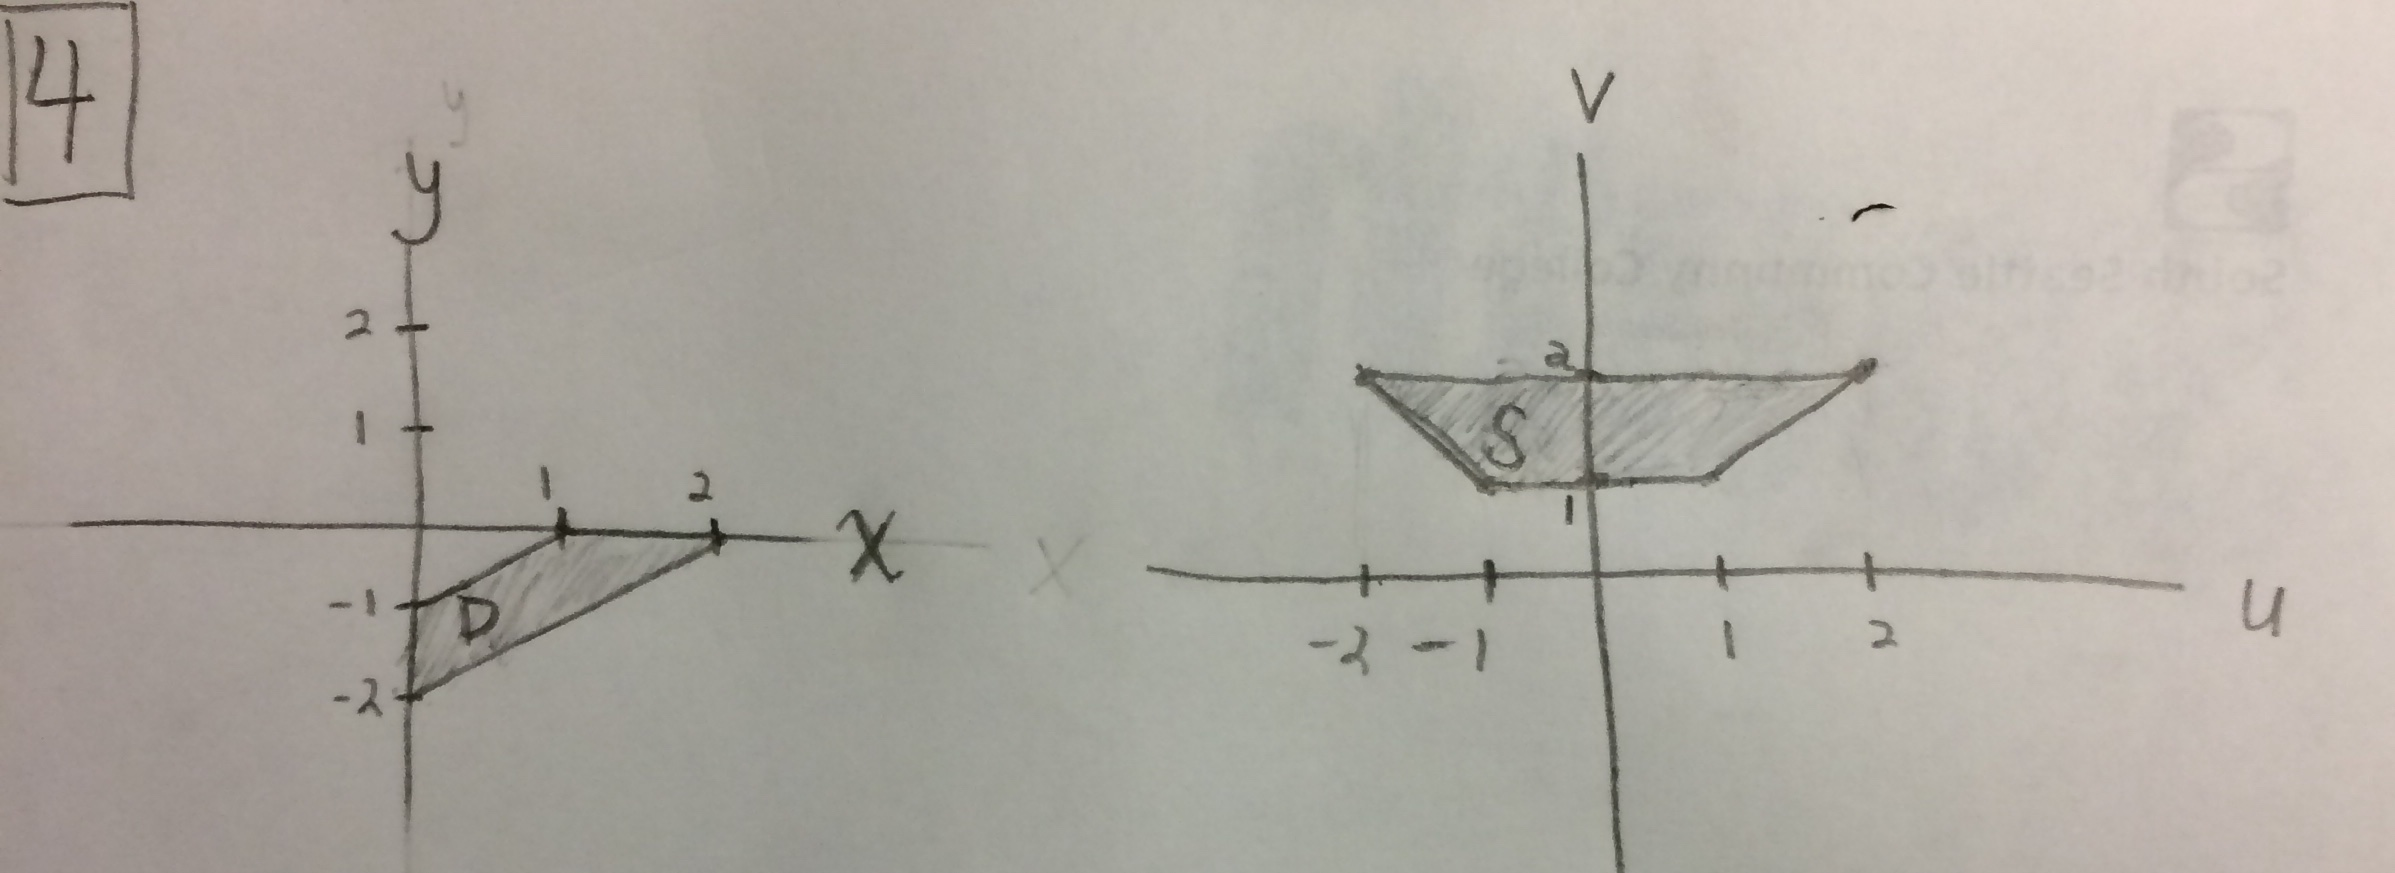
\includegraphics[scale= 0.15]{P4}
\\

(c)

\begin{align*}
\int \int_D e^{\frac{x+y}{x-y}} \: dA & = \int \int_S \frac{1}{2} e^{\frac{u}{v}} \: du \, dv \\
& =\frac{1}{2} \int_{1}^{2} \int_{-v}^{v} e^{\frac{u}{v}} \: du \, dv \\
& =\frac{1}{2} \int_{1}^{2} \left(ve^{\frac{u}{v}}\right) \Bigr\rvert_{-v}^{v} \: dv \\ 
& = \frac{1}{2} \left(e - \frac{1}{e} \right)\int_{1}^{2} v \: dv \\
& = \frac{1}{4} \left(e - \frac{1}{e} \right) v^2 \Bigr\rvert_{1}^{2} \\
& = \frac{3}{4} \left(e - \frac{1}{e} \right) \:.
\end{align*}
5. (a) Compute $\int \int_D \sqrt{x^2 + y^2} \: dx \, dy$ on $ D = \{(x,y) : 1 \leq x^2 + y^2 \leq 9, \: y \geq 0 \} $ by changing to polar coordinates. 
\\

Let $ x = rcos(\theta) \quad y = rsin(\theta)$. Then \begin{align*}
\int \int_D \sqrt{x^2 + y^2} \: dx \, dy &= \int_{0}^{\pi} \int_{1}^{3} \sqrt{r^2} \, r \, dr \, d\theta \\ & = \left(\theta \Bigr\rvert_{0}^{\pi} \right) \left( \frac{r^3}{3} \Bigr\rvert_{1}^{3} \right) \\
& = \frac{26\pi}{3} \:.
\end{align*}

Here are the sketches of the two regions of integration:

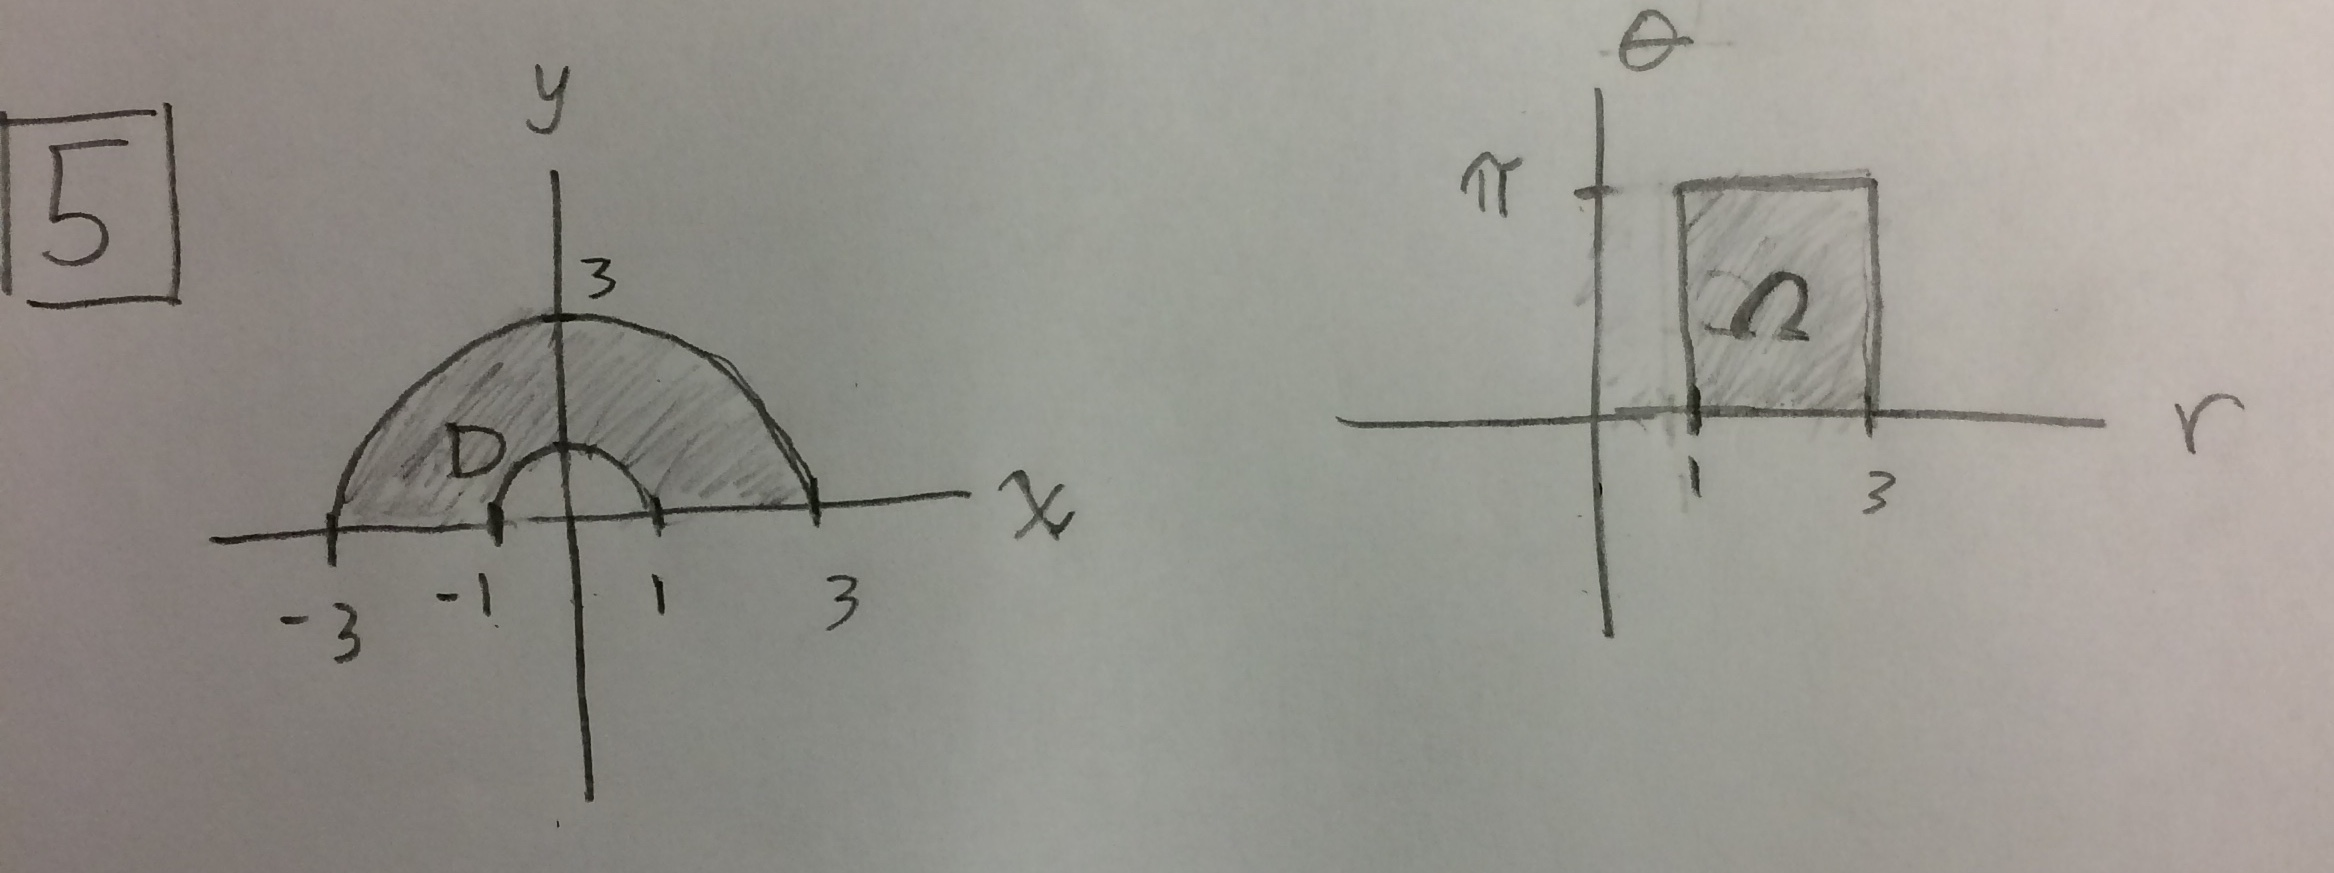
\includegraphics[scale= 0.15]{P5}
\\


(b) Compute
$$\int \int_D sin(\sqrt{x^2 + y^2}) \: dx \, dy \;on\; D = \{(x,y) : \pi^2 \leq x^2 + y^2 \leq 4\pi^2\} $$

Using polar coordinates we have
\begin{align*}
\int \int_D sin(\sqrt{x^2 + y^2}) \: dx \, dy & = \int_{0}^{2\pi} \int_{\pi}^{2\pi} rsin(r) \, dr \, d\theta \\
& = 2\pi \int_{\pi}^{2\pi} rsin(r) \, dr \\
& = 2\pi \left[-rcos(r) \Bigr\rvert_{\pi}^{2\pi} + \int_{pi}^{2\pi} cos(r) \, dr \right] \\
& = 2\pi \left[ -2\pi - \pi + sin(2\pi) - sin(\pi) \right] \\
& = -6\pi^2.
\end{align*}

Sketches of the regions of integration were not requested for this last problem but note that the transformation of the annular region D in Cartesian coordinates becomes a square in $(r,\theta)$ coordinates (similar to the first part of problem 5 except the annulus is a full ring this time).
\end{document}